% Prepinace pre figure:
% h=approximately here
% t=top of page
% b=bottom of page
% p=on special page
% H=precisely here
\newcommand{\InsertCode}[2]{\begin{figure}[#1]\input{#2}\end{figure}}

\newcommand{\Code}[1]{\texttt{#1}}

\chapter{Overview of database frameworks in java \label{frameworks}}

In this chapter, we will analyse some of database frameworks that are mainly used
to connect to databases and load (or store) data to (or from) java applications
as this is main topic of our work, which is identifying database type
and all the places places when application communicate with that database.

All of the frameworks has many advanced features that does not fit our topic.
We will try to follow one example of loading class \Code{DatabaseValue} as can be seen in
example \ref{code:model} from database structured as in \ref{code:db}.

\InsertCode{h}{code/model}

TODO RE model databaze:
\begin{lstlisting}[caption={Example of database}, label={code:db}]
TABLE T
ID  | VALUE
1   | A
2   | B
... | ...
\end{lstlisting}







\section{JDBC \label{frameworks:jdbc}}

For accessing database in java application, there exists standard Java Database Connectivity (JDBC) API,
which is described in more detail in \citet{JDBC_OVERVIEW}.

Database vendors ususally provide JDBC API implementation. API is generic, so
there should be no difference for connecting to different database types.

There are few interfaces in \citet{java.sql} package controlling database calls.
\begin{itemize}
  \item \Code{Connection}
  \item \Code{Statement}, \Code{PreparedStatement}, \Code{CallableStatement}
  \item \Code{ResultSet}
\end{itemize}

\Code{Connection} object should hold database connection and through this connection
database queries can be executed using any of \Code{Statement} calls.
When data are returned to application from statement, it is done through \Code{ResultSet}.

Getting connection to database is through \Code{DriverManager}, or from JDBC 2.0
it can be done using \Code{DataSource} and it is now the preferred way of connecting to database.
Example \ref{code:datasource} shows how \Code{DataSource} can be created for Oracle database
that is listening on url \Code{jdbc:oracle:thin:@//192.168.0.16:1521/orcl}
and \Code{User} user and \Code{Password} password is used when connecting to it.

Calls of \Code{createDataSource()} would be used in next examples.

\InsertCode{h}{code/datasource}
\InsertCode{H}{code/jdbc}

JDBC example \ref{code:jdbc} shows how can be done loading data from \Code{DataSource} (as in \ref{code:datasource}).
On line \ref{code:jdbc:connection}, connection to database is created.
Then on lines \ref{code:jdbc:prepareStatement:begin}--\ref{code:jdbc:prepareStatement:end}
database query is created to select just rows matching \Code{id} argument.
The query is then executed on line \ref{code:jdbc:executeQuery} and then
result is mapped from \Code{ResultSet} to our \Code{DatabaseValue} model and then it is returned on line \ref{code:jdbc:return}.

As you can see, there is huge amount of boilerplate code (catch-finally blocks) for closing every JDBC API object,
as exceptions can be thrown from almost all calls and we need to free all database resources that we do not need anymore.

From Java 7, try-with-resources can be used with result, that all finally blocks can be removed - resources
(Connection, PreparedStatement, ResultSet) are automatically closed after finishing block.
This is ilustrated in example \ref{code:jdbc-try-with-resources}.

\InsertCode{h}{code/jdbc-try-with-resources}




\section{Spring JDBC Framework \label{frameworks:jdbcTemplate}}
\citet{SpringJDBC} Framework is extension above JDBC API and tries to help users to code only
parts with application logic and it removes much of the boilerplate code.
From next list, only italicized lines need to be coded by user:
\begin{itemize}
  \item Define connection parameters
  \item Open the connection
  \item \textit{Specify the statement}
  \item Prepare and execute the statement
  \item Set up the loop to iterate through the results (if any)
  \item \textit{Do the work for each iteration}
  \item Process any exception
  \item Handle transactions
  \item Close the connection   
\end{itemize}

Before Java 7, coding in standard JDBC tend to be errorneus because of forgetting to close
database resources and boilerplate code does not help in readability of code
(as could be seen in example \ref{code:jdbc}). These problems are removed using Spring JDBC Framework,
as illustrate example \ref{code:jdbcTemplate}. It shows, how can be loaded single row from database.
We can see, that mappings are the same in standard JDBC and Spring JDBC examples.
Framework handles all boilerplate code around and result is returned after processing single line \ref{code:jdbcTemplate:return}.


\InsertCode{h}{code/jdbcTemplate}





\section{MyBatis \label{frameworks:myBatis}}

\citet{MyBatis} framework is one of Object-Relational Mapping (ORM) frameworks.
It uses JDBC API to communicate with database, but in almost all cases, there is no need
to work with low level JDBC.

Unlike other ORM frameworks, it does not map java objects to database tables, but java methods
to SQL statements. All communication with database is always through methods in user created interfaces.
SQL statements are stored in XML files or annotations in these interfaces.

In subsection \ref{mybatis:mapper} we show examples of \Code{Mapper} interface definitions,
which can be done by annotations or using XML mapper files.
Logic that is made in background by MyBatis by calling these interfaces
is same as we could see in previous JDBC or Spring JDBC examples,
when from some database connection \Code{PreparedStatement} is created.
Next, method argument \Code{id} is set and query is executed.
After execution, from \Code{ResultSet} are values of columns
mapped to object attributes and object is returned.

Subsection \ref{mybatis:configuration} shows how database
configuration can be made and subsection \ref{mybatis:run}
shows how data can be loaded from such a database.



\subsection{MyBatis Mapper definition \label{mybatis:mapper}}

\InsertCode{h}{code/mybatis-interface-annotations}

Example \ref{code:mybatis:interface:annotations} uses annotations to store definitions of both query and mapping.
Query is defined using \Code{@Select} annotation on line \ref{code:mybatis:interface:annotations:query}
and mapping is defined using \Code{@Results} and \Code{@Result} annotations.

\InsertCode{h}{code/mybatis-interface-xml}
\InsertCode{H}{code/mybatis-mapper-xml}

Snippets \ref{code:mybatis:interface:xml} and \ref{code:mybatis:mapper:xml} contains definitions
of plain interface which has query and mapping stored in XML mapper file.
Query is located on line \ref{code:mybatis:mapper:xml:query} in \Code{<select>} tag.
Tag contains reference to correct \Code{resultMap} mapping on lines
\ref{code:mybatis:mapper:xml:mapping:begin}--\ref{code:mybatis:mapper:xml:mapping:end}.



\subsection{MyBatis Configuration \label{mybatis:configuration}}

MyBatis framework uses interface \Code{SqlSessionFactory} for creating database connections.
Factory can be created using both Java and XML files.

\InsertCode{h}{code/mybatis-sessionFactory-java}

Example \ref{code:mybatis:sessionFactory:java} shows how configuration can be done in Java.
We set \Code{DataSource} reference to \Code{Environment} class on line \ref{code:mybatis:sessionFactory:java:dataSource}.
\Code{JdbcTransactionFactory} was used to handle database transactions.
On line \ref{code:mybatis:sessionFactory:java:addMapper} mapper class is registered to be known by MyBatis
and next \Code{SqlSessionFactory} is created.

\InsertCode{h}{code/mybatis-sessionFactory-xml}
\InsertCode{H}{code/mybatis-configuration-xml}

The same can be also done using XML configuration file.
\Code{SqlSessionFactory} is created in snippet \ref{code:mybatis:sessionFactory:xml}
after loading configuration file on line \ref{code:mybatis:sessionFactory:xml:file}.

XML configuration file \ref{code:mybatis:configuration:xml} configures \Code{DataSource} on lines
\ref{code:mybatis:configuration:xml:dataSource:begin}--\ref{code:mybatis:configuration:xml:dataSource:end}
and \Code{Mapper} class is registered on line \ref{code:mybatis:configuration:xml:mapper}.



\subsection{Loading data from database using MyBatis \label{mybatis:run}}

As we know how to configure database connections and how to define mappers,
in example \ref{code:mybatis} we show how data can be loaded.

On line \ref{code:mybatis:getMapper}, the implementation of \Code{Mapper} interface
that was made by MyBatis is returned and on next line \ref{code:mybatis:return} database query is executed.

\InsertCode{h}{code/mybatis}



\section{Kafka}

Apache Kafka \citet{Kafka} is a distributed streaming platform.
It means, that application can publish or subscribe records and
process them, as they occurs.

Application that want to publish some records, it sends them to server
and data are send to all subscribers of the same \textit{topic}
(for detailed info see \ref{frameworks:kafka:background}).

Kafka has four core APIs:
\begin{itemize}
  \item The \textbf{Producer API} allows an application to publish
    a stream of records to Kafka topics
  \item The \textbf{Consumer API} allows an application to subscribe
    to topics and process the stream of records produced to them
  \item The \textbf{Streams API} allows an application to act as a stream processor,
    consuming an input stream from topics and producing an output stream to output topics,
    effectively transforming the input streams to output streams
  \item The \textbf{Connector API} allows building and running reusable producers or consumers
    that connect Kafka topics to existing applications or data systems.
    For example, a connector to a relational database might capture every change to a table. 
\end{itemize}

Figure \ref{frameworks:kafka:api} shows, how client applications can communicate with Kafka server
using Kafka APIs.

\begin{figure}[h]
  \center
  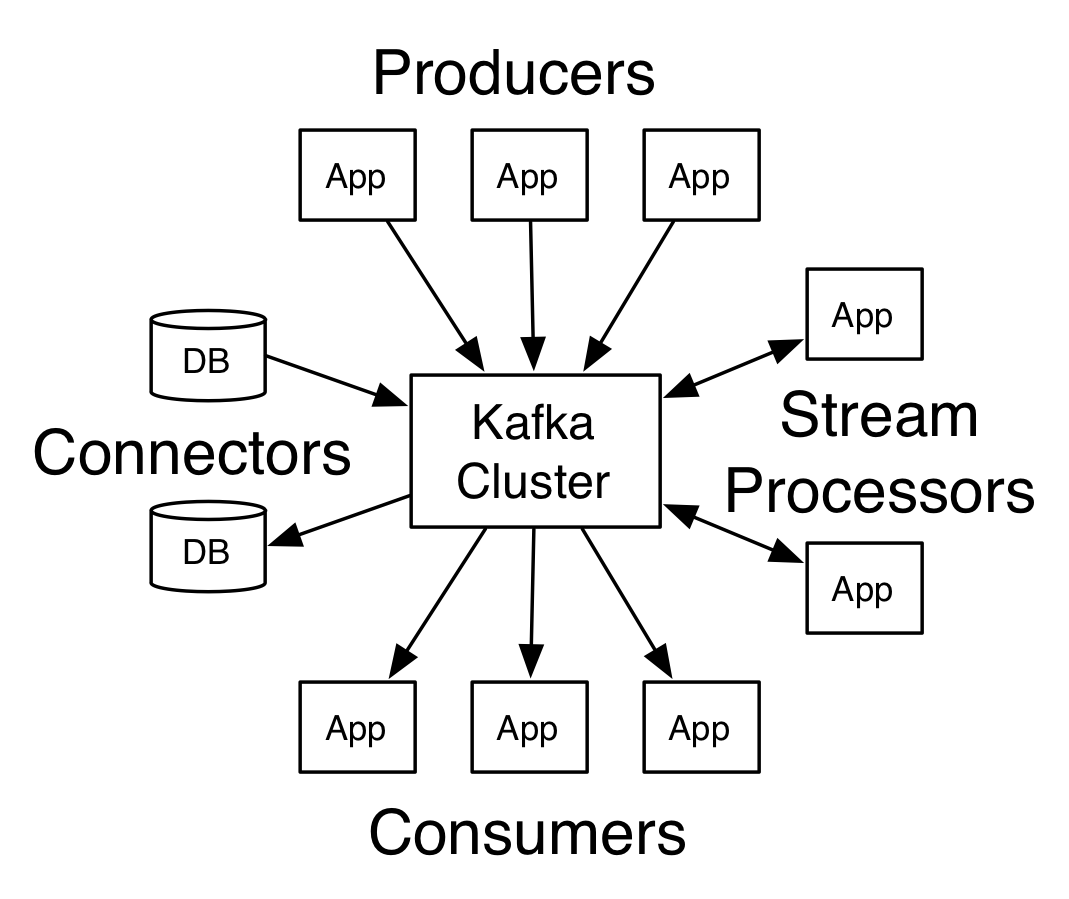
\includegraphics[width=100mm]{img/kafka-apis.png}
  \label{frameworks:kafka:api}
  \caption{Applications using differend kinds of Kafka APIs}
\end{figure}



\subsection{Kafka background \label{frameworks:kafka:background}}

Kafka can be run as a cluster on one or more servers.
Each cluster stores stream of records in categories that are called topics
and each record consist of a key, value and timestamp.

Topics can be compared to the database tables. Application that is publishing topic
writes to that table and the one that subscribe topic reads that data.

Kafka topics can be also partitioned, so distributed computations can be made
on them - each partition can be handled by different server/producer/consumer.
Each partition is an ordered, immutable sequence of records that is
continually appended to.

The Kafka cluster durably persists all published records (whether or not they have been consumed)
using a configurable retention period. For that period, any consumer can access
to any record published, as can be seen in figure \ref{frameworks:kafka:partitions}.

\begin{figure}[h]
  \center
  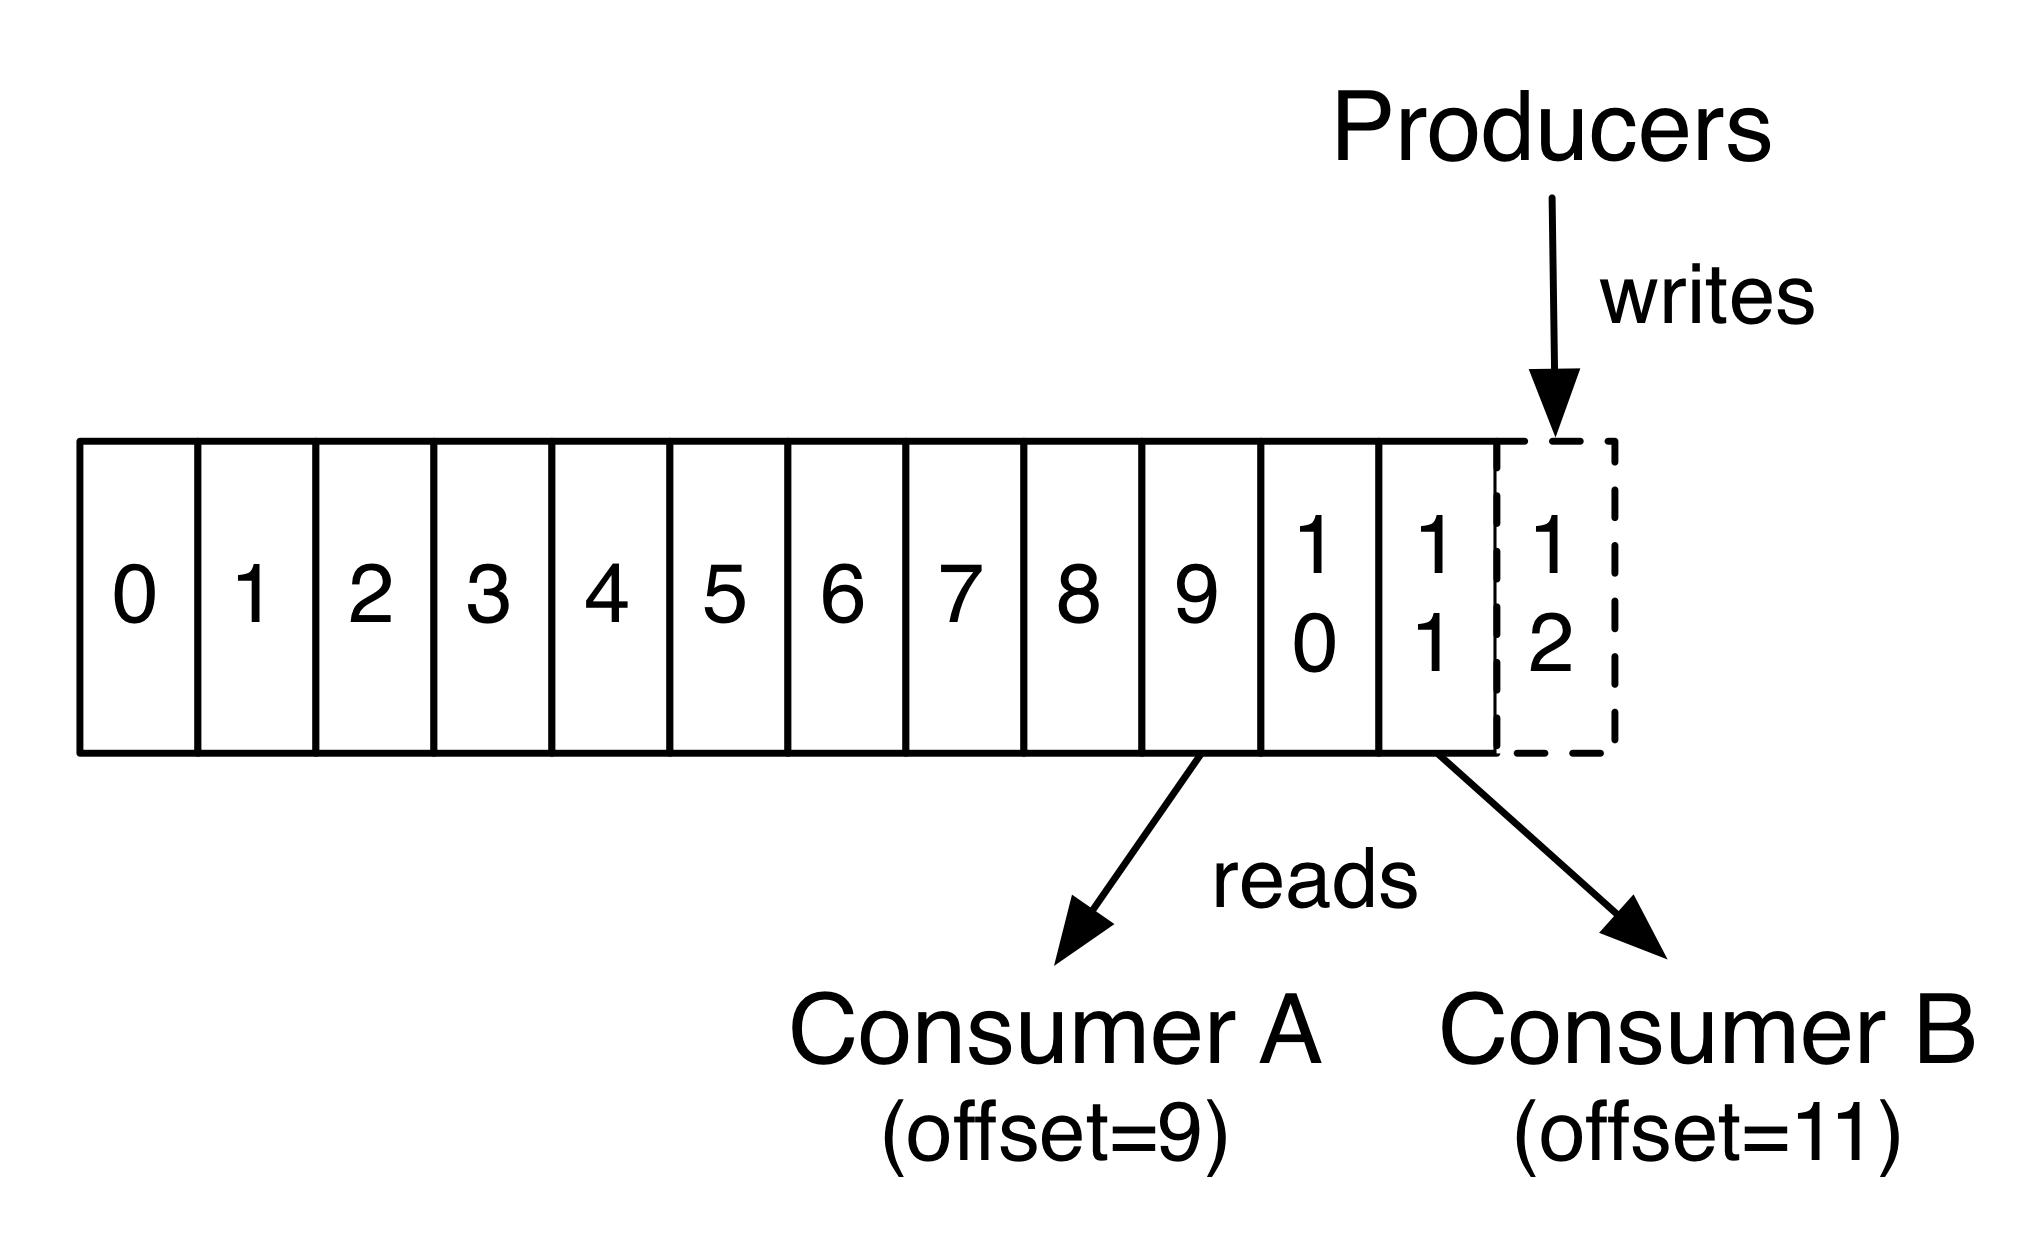
\includegraphics[width=100mm]{img/kafka-partitions.png}
  \label{frameworks:kafka:partitions}
  \caption{Producers are appending new records to Kafka partition and Consumers accessing them}
\end{figure}

In our work, we will be concerned with Producer and Consumer APIs,
because other two are much more advanced to use.



\subsection{Kafka Producers and Consumers}

\InsertCode{h}{code/kafka-producer}
\InsertCode{h}{code/kafka-consumer}

Structure of data in records can be arbitrary. Application just need to handle
correct transformation of used Java object to (or from) byte array using
\Code{Serializer<T>} (or \Code{Deserializer<T>}) objects.
However, for our data lineage problem, feature of serializing
and deserializing objects is unimportant. There is always one
source/target - the byte array. There, we cannot distinguish values
that belong to same attribute that was written to and then read from that array\footnote{
  As could be done in case of databases, where rows were divided into columns.
}.

Using Producer API, application can create new records and send them to topic of Kafka server.
After creating \Code{KafkaProducer} with some configuration as in \ref{code:kafka:producer},
records can be send to server by calling \Code{send()} method.

With Consumer API, application can handle new records that are arriving from server.
One has to create configured \Code{KafkaConsumer}, subscribe to some topics
and wait for new records. This is illustrated in snippet \ref{code:kafka:consumer}.
On line \ref{code:kafka:consumer:properties}, kafka server url is configured.
Then consumer registers itself to receive records in topic \Code{Topic}
on line \ref{code:kafka:consumer:subscribe} and on line \ref{code:kafka:consumer:poll}
kafka is queried for data. There is some maximal time limit, for which kafka waits for
new records to arrive (in our case 1 second) and then it returns them.







